\chapter{O modelo abstrato de estimação do juros da dívida técnica}
\label{estimacao:juros}

Neste capítulo definiremos um modelo para estimação dos juros da dívida técnica. Nesse modelo, os juros serão considerados como a diminuição, causada pela dívida técnica, da produtividade dos projetos de desenvolvimento de software. Inicialmente, iremos descrever a versão de alto nível desse modelo e em quais ideias ele está baseado. Em seguida, forneceremos uma descrição de quais passos são necessários para que seja criada uma instância desse modelo. 



\section{Introdução}



Tradicionalmente, os juros da dívida técnica são definidos como o conjunto das dificuldades adicionais, causadas pela existência da dívida, para realizar as atividades de desenvolvimento de software. Caso a dívida técnica não estivesse presente, essas dificuldades não existiriam. Nesta pesquisa, sugerimos uma nova perspectiva para analisar os juros da dívida técnica e, assim, permitir seu gerenciamento: considerá-los como a causa de uma diminuição da produtividade dos projetos. 

Quanto mais juros um projeto tem, menor a produtividade real, quando comparada à obtida em um cenário onde não houvesse dívida técnica. Essa redução acontece, pois mais recursos terão de ser utilizados para se atingirem os mesmos objetivos. Vamos ilustrar essa  degradação na produtividade com um exemplo: 

\begin{tcolorbox}
Uma empresa de desenvolvimento de software resolve iniciar um projeto para o desenvolvimento de algumas novas funcionalidades para um sistema de vendas existente. Ao realizar uma análise de viabilidade, o time responsável descobre que o código atual do sistema apresenta uma documentação insuficiente, problemas de arquitetura e design e quantidade de testes unitários não compatível com o nível de qualidade esperado para o projeto. O time conclui, corretamente, que haverá uma série de dificuldades adicionais para a conclusão do projeto. 
\end{tcolorbox}

Nesse exemplo, fica claro que a produtividade do time seria melhor caso esses problemas identificados não existissem. Ou seja, menos recursos teriam de ser gastos para alcançar os mesmos objetivos. Os problemas encontrados são as dívidas técnicas do software que foram sendo adquiridas com o passar do tempo. As dificuldades para se realizar o projeto de adição das funcionalidades adicionais são os juros causados por essas dívidas. Observando o exemplo fornecido, proporemos um modelo, no qual a estimativa dos juros da dívida técnica será calculado como a diferença de produtividade entre dois cenários: um com dívida técnica, semelhantemente ao exemplo fornecido, e um cenário onde essas dívidas técnicas não existam. Como discutiremos mais à frente, na verdade, o cenário onde não existe dívida é inalcançável. O que usaremos será uma aproximação em que a dívida técnica seja muito baixa. 


\section{Avaliação da produtividade dos projetos de software}
\label{modelo_de_estimacao_produtividade}

O termo produtividade é usado para descrever a proporção entre o valor dos recursos utilizados em um processo e o valor do que é efetivamente produzido. Os recursos aplicados são chamados de entradas, enquanto os resultados do processo são chamados de saídas. O problema de medir a produtividade de um processo pode ser resumido em duas partes:

\begin{enumerate}
\item Identificar as entradas e as saídas.
\item Quantificar  as entradas e saídas de tal forma que a relação entre elas possa ser calculada
\end{enumerate} 

O processo mais eficiente é aquele no qual mais valor (saídas) é produzido utilizando menos recursos (entradas).

Existe uma série de desafios para identificar e quantificar as entradas e saídas do processo de desenvolvimento de software. Devido à inerente complexidade desse processo, existem diversas possibilidades para quais serão as entradas e saídas a serem incluídas na análise de produtividade. A quantidade de homens/hora e a quantidade de linhas de código produzidas são métricas normalmente utilizadas como entrada e saída respectivamente.  Entretanto, essas métricas, apesar de poderem ser consistentemente medidas, são demasiadamente imprecisas, já que existem diversos outros fatores relevantes conforme mostrado no estudo de MacCormack et al. \cite{maccormack2003trade}. No caso da quantidade de homens/hora, por exemplo, um outro fator importante é o nível de experiência das pessoas envolvidas. A hora de um colaborador inexperiente naturalmente será menos valiosa do que a hora de um com mais experiência. Semelhantemente, a quantidade de linhas de código produzidas, apesar de muito utilizada, também é uma métrica imprecisa já que não inclui uma quantificação do valor dessas linhas de código.  É possível que uma grande quantidade de linhas de código seja criada para realizar uma atividade, porém, essa mesma atividade possa ser desenvolvimento com uma quantidade bem menor. Além desses dois exemplos, existem outras entradas e saídas que podem ser utilizadas em modelos de medição de produtividade conforme mostrado por Hernández-López et al.,\cite{hernandez2015productivity}. Podemos observar que não existe uma forma totalmente precisa para se avaliar a produtividade dos processos de desenvolvimento de software. Isso se dá não apenas pela existência de diversas medidas possíveis como também devido aos aspectos subjetivos dessas medidas. 

\subsection{Modelos baseados em expectativa de produção}

Para medir a produtividade no nosso modelo de estimação, utilizamos uma proposta de Kitchenham e Mendes \cite{kitchenham2004software}. Nesse trabalho os autores sugerem um modelo onde a produtividade de um processo de desenvolvimento de software é avaliada comparando o esforço estimado para a realização de um determinado projeto com o esforço efetivamente gasto. Essa relação é representada pela equação ~\ref{eq:model}. O esforço estimado, representado pela variável \textit{AdjustedSize}, é calculado por meio de uma regressão linear múltipla utilizando dados históricos de projetos similares. A variável $Effort$ é o esforço efetivamente gasto para a realização do projeto. Se a variável $Productivity$ for maior que 1 quer dizer que o projeto foi realizado com menos esforço do que o esperado levando-se em consideração os dados dos projetos semelhantes.
 
 
 

\begin{equation}
\label{eq:model}
  Productivity = AdjustedSize/Effort
\end{equation}


O modelo descrito na equação \ref{eq:model} não determina quais medidas serão utilizadas para quantificar as variáveis $AdjustedSize$ e $Effort$. Isso é esperado já que essas medidas são diferentes para cada domínio da aplicação sendo desenvolvida. Os autores fornecem um exemplo da aplicação do modelo em um projeto de desenvolvimento web. Nesse exemplo, são utilizados o número de páginas, o número de imagens e o número de funcionalidades da aplicação como medidas para estimar o esforço. 

Apesar da viabilidade dessa estratégia, os autores  concluem que calcular a produtividade esperada, utilizando os  fatores associados, é uma atividade complexa e que também não pode ser feita com precisão absoluta \cite{petersen2011measuring}.

Devido à importância, nesta pesquisa, do modelo de produtividade representado pela equação \ref{eq:model}, forneceremos um exemplo de como ele deve ser utilizado. Na Tabela \ref{tab:examplo_aplicacao_modelo_produtividade} há a quantidade de linhas produzidas e a quantidade de desenvolvedores de três projetos fictícios. Podemos estimar, utilizando os dados desses três projetos, qual seria a quantidade de desenvolvedores necessários para produzir a quantidade de linhas de código do projeto. Essa estimação é realizada por meio de uma regressão linear\cite{degroot2012probability} tendo como variável explicativa o número de linhas de código e como variável explicada o número de desenvolvedores. Realizando essa regressão linear, podemos calcular os valores ajustados para o número de desenvolvedores.

No exemplo da Tabela \ref{tab:examplo_aplicacao_modelo_produtividade}, podemos observar que o projeto A envolveu cinco desenvolvedores, porém, o número esperado, tendo como base os dados dos outros projetos, seria 5,33.  portanto, o projeto A conseguiu produzir 15.000 linhas de código com uma quantidade menor do que  a esperada de desenvolvedores. A razão entre a quantidade esperada e a quantidade real de desenvolvedores é a produtividade do projeto, de acordo com a equação \ref{eq:model}. Por outro lado, o projeto B tem uma quantidade de desenvolvedores maior do que a esperada. Com isso, a produtividade desse projeto foi menor do que 1, o que o leva a ser considerado um projeto menos produtivo do que o projeto A.

\begin{table}[H]
\centering
\begin{tabular}{lllll}
\hline
\textbf{Projeto} & \textbf{Linhas de código} & \textbf{Nº Desen.} & \textbf{Nº  Desen. ajustado}  & \textbf{Produtividade}\\ \hline
A                & 15.000                     & 5       & 5.33  &        1,06          \\ \hline
B                & 20.000                     & 8       & 7.33   &       0,91         \\ \hline
C                & 25.000                     & 9        & 9.33    &      1,03         \\ \hline
\end{tabular}
\caption{Quantidade de linhas de código, número de desenvolvedores, número de desenvolvedores ajustado e produtividade de três projetos de software fictícios.}
\label{tab:examplo_aplicacao_modelo_produtividade}
\end{table}





\section{O modelo de estimação dos juros da dívida técnica}
\label{modelo_abstrato}


O nosso modelo de estimação dos juros tem como base a existência de dois cenários nos quais um mesmo projeto de software pode ser desenvolvido:

\begin{itemize} 
\item  \textbf{sem dívida técnica}. Nesse cenário, a produtividade de um projeto de software é a melhor possível com os recursos disponíveis, ou seja, levando-se em consideração todo o contexto no qual o projeto é desenvolvido, a produtividade obtida é a melhor que poderia ser alcançada. 
\item \textbf{com dívida técnica}. Esse cenário é idêntico ao cenário \textbf{sem dívida técnica}, exceto por uma diferença: existem dívidas técnicas.   Todas as outras variáveis relacionadas com o contexto do projeto são exatamente as mesmas. Ou seja, as atividades a serem realizadas são as mesmas e com o mesmo nível de complexidade.
\end{itemize}

  

É importante notar que o cenário totalmente sem dívida técnica nunca existirá já que não é possível a existência de um software sem nenhuma dívida técnica. Temos algumas razões para afirmar a inexistência de projetos sem nenhuma dívida técnica. A primeira delas é o fato de que a própria identificação do que é ou não uma dívida técnica é subjetiva e muitas vezes intangível. A segunda razão é associada às dívidas técnicas de tecnologia. Com o passar do tempo uma tecnologia vai se tornando obsoleta e continuar a utilizá-la pode trazer esforços adicionais. Com isso, devido à contínua criação de novas tecnologias, é impossível garantir que não haja algum tipo de obsolescência. 


Vamos revisitar agora o exemplo anteriormente fornecido neste capítulo incluindo as definições dos dois cenários de desenvolvimento e outros conceitos já introduzidos: 

\begin{tcolorbox}

Um determinado projeto de desenvolvimento que consistia em adicionar um conjunto de novas funcionalidades a um sistema já existente foi realizado em um cenário \textbf{com dívida técnica}. Ou seja, esse sistema existente possuía um número  $D$ de dívidas técnicas.  Esse projeto adicionou uma quantidade $S$ de funcionalidades ao sistema. Para obter o resultado  $S$  foi utilizada  uma equipe de desenvolvimento de software de tamanho $E$ obtendo uma produtividade $Y$.   Com isso, a produtividade $Y$ do projeto pode ser calculada de acordo com a equação \ref{eq:juros_1}. Por meio da equação \ref{eq:juros_1}, representamos a degradação da produtividade causada pela existência da dívida técnica $D$. Quanto maior $D$, menor será a produtividade do projeto.

\begin{equation}
\label{eq:juros_1}
Y =  \frac{S}{D*E}
\end{equation}

\end{tcolorbox}




Imagine que seja possível que esse mesmo projeto pudesse ser realizado novamente pela mesma equipe e em um contexto exatamente igual, porém sem que a equipe pudesse lembrar da primeira execução e usar o que aprendeu nela. Além disso, nesta segunda execução, a dívida técnica do projeto não existe. Ou seja, o projeto dessa vez foi realizado em um cenário de \textbf{sem dívida técnica}. Logo, a produtividade do time de desenvolvimento será outra que chamaremos de $\overline{Y}$. A produtividade  $\overline{Y}$ pode ser calculada utilizando a Equação \ref{eq:juros_2}. 

É esperado que  a produtividade $\overline{Y}$ será melhor do que a produtividade  $Y$ já que a única diferença entre os dois cenários, nesse exemplo fictício,  é a existência ou não de dívida técnica. Sem a dívida técnica, o time terá mais facilidade para desenvolver as funcionalidades do projeto e com isso elas serão desenvolvidas em um menor tempo aumentando, assim, a produtividade. Observando esse exemplo fictício podemos inferir a Equação \ref{eq:juros_3} em que $J$ são os juros da dívida técnica que foram pagos durante a execução do projeto de desenvolvimento no cenário de \textbf{com dívida técnica}. \textit{\textbf{Note que, para este exemplo fictício,  $J$ não  é uma estimativa dos juros, ao invés disso, é um valor exato}}.  

Esse exemplo fictício obviamente não pode ser reproduzido exatamente como descrito. Um motivo é a impossibilidade de executar o mesmo projeto duas vezes com o mesmo time sem que a segunda execução seja facilitada pelas experiências obtidas pela primeira. Outro motivo é a impossibilidade de se remover totalmente a dívida técnica $D$ do sistema existente. Contudo, esse exemplo apresenta-se útil como uma argumentação lógica para uma estratégia onde possa ser encontrado um valor aproximado para $J$ em situações reais.

\begin{equation}
\label{eq:juros_2}
\overline{Y} =  \frac{S}{E}
\end{equation}


\begin{equation}
\label{eq:juros_3}
J = \overline{Y} - Y
\end{equation}

\subsection{Estimação dos juros por aproximação}
\label{estimacao_juros_por_aproximacao}

Conforme descrito anteriormente, não podemos calcular precisamente os juros da dívida técnica utilizando a Equação \ref{eq:juros_3}. Porém, utilizaremos essa fórmula e a situação fictícia que descrevemos como uma base lógica para o cálculo de uma estimativa dos juros da dívida técnica. Para isso, precisamos de valores estimados para $Y$ e $\overline{Y}$. Nossa estratégia será a de estimar o valor de $Y$ utilizando os projetos no cenário  \textbf{com dívida técnica} e o valor de $\overline{Y}$ utilizando os projetos no cenário  \textbf{sem dívida técnica} da seguinte forma:

\begin{enumerate}
\item Selecionamos um projeto A que tenha um nível normal de dívida técnica.  A produtividade desse projeto será a variável $Y$ da equação  \ref{eq:juros_3}.
\item Selecionamos um projeto B  que seja muito semelhante ao projeto A, porém tenha um nível de dívida técnica muito baixo, ou seja, esteja no cenário  \textbf{sem dívida técnica}. A produtividade desse projeto será a variável $
\overline{Y}$ da equação  \ref{eq:juros_3}. O limite de dívida técnica  que um projeto pode ter e ainda ser considerado pertencente a esse cenário dependerá do contexto desse projeto. 
\item Calculamos um valor estimado para $J$ usando a equação \ref{eq:juros_3}.
\end{enumerate}

Com isso, estamos simulando a remoção da dívida $D$ do projeto A e criando uma aproximação da realização do projeto A sem a existência de dívida técnica, o que nos permite a estimação do valor de $J$, que representa os juros da dívida técnica do projeto A.

Como veremos no nosso estudo de caso do Capítulo \ref{cap_estudo_caso}, podemos usar mais de um projeto para representar as variáveis $Y$  e  $\overline{Y}$ da seguinte forma:

\begin{enumerate}
\item Definimos um grupo $G$ de projetos que sejam todos semelhantes entre si.
\item Dividimos o grupo $G$ em duas partições: 
\begin{enumerate}
\item[$P_1$] Projeto no cenário \textbf{sem dívida}
\item[$P_2$] Projetos no cenário \textbf{com dívida}.
\end{enumerate}
\item Atribuímos a produtividade média dos projetos na partição $P_1$ à variável $\overline{Y}$.
\item Atribuímos a produtividade média dos projetos na partição $P_2$ à variável $Y$.
\item Calculamos um valor médio para $J$ usando a equação \ref{eq:juros_3}. Nesse caso, $J$ representa a média de juros da dívida técnica dos projetos na partição $P_2$
\end{enumerate}
 
 \subsection{Abstração do modelo}
 
Nosso modelo de estimação dos juros é um modelo abstrato.  Não há uma definição de quais métricas serão utilizadas tanto para a estimação da dúvida quanto para a estimação da produtividade.  Para que esse modelo possa ser aplicado, é necessário que exista uma definição precisa a respeito de quais métricas serão utilizadas para avaliar a produtividade e qual processo será realizado para estimar os juros da dívida técnica.  Entretanto essas definições dependem das características dos projetos avaliados. Por exemplo, o conjunto de dívidas técnicas em um projeto no qual o paradigma de desenvolvimento seja o orientado a objetos é diferente do conjunto de dívidas técnicas de um projeto que utilize o paradigma funcional. Por isso, essas definições, nessárias para aplicação do modelo proposto, precisam ser feitas de acordo com o contexto. Ou seja, para aplicar o modelo, é necessário criar uma instância dele conforme ilustrado na Figura \ref{fig:cap_metodo_niveis_abstracao}.


  \begin{figure}[H]
  \centering
  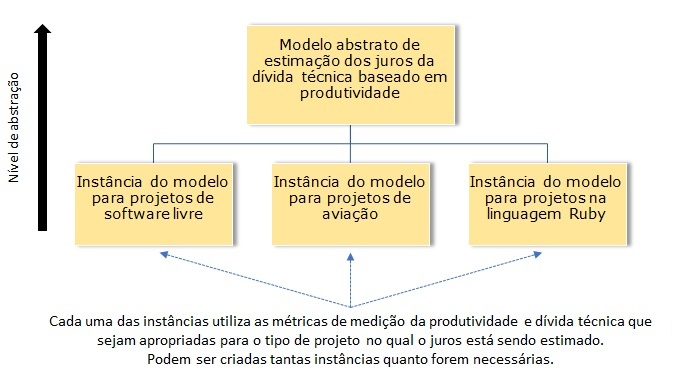
\includegraphics{capitulo_metodo/NiveisDeAbstracoesModelo.jpg} 
  \caption{Níveis de abstração do modelo de estimação dos juros da dívida técnica. }
  \label{fig:cap_metodo_niveis_abstracao} 
\end{figure}


 
 \section{Criação das instâncias do modelo de estimação dos juros da dívida técnica}
  
Para instanciar o modelo de estimação é necessário definir certas métricas que serão utilizadas para avaliar a produtividade dos projetos. Além disso, será necessário definir como agrupar os projetos semelhantes como também particionar cada um desses grupos de forma a separar os projetos nos cenários \textbf{com dívida técnica} e \textbf{sem dívida técnica}. A tabela \ref{cap_modelo_tabela_resumo_passos} resume todas as definições que precisam ser feitas para a instanciação do modelo para a estimação dos juros da dívida técnica.  A seguir descreveremos cada uma dessas atividades.
 
 
 \begin{table}[H]
 \centering
\caption{Atividades necessárias para a criação de um modelo concreto de estimação dos juros da dívida técnica específico.}
\label{cap_modelo_tabela_resumo_passos}
\begin{tabular}{l|l}
\hline
 & \multicolumn{1}{c}{Atividade}                                \\ \hline
1  & Seleção das métricas que representam as entradas do processo  \\ \hline
2  & Seleção das métricas que representam as saídas do processo    \\ \hline
3  & Definição do método de agrupamento dos projetos semelhantes   \\ \hline
4  & Definição do método de particionamento dos grupos de projetos \\ \hline
\end{tabular}
\end{table}


\subsection{Seleção das métricas que representam as entradas do processo}

Em um modelo de avaliação de produtividade de um processo, as entradas representam aquilo que é gasto para que o resultado do processo seja alcançado. Nessa etapa, são definidas quais entradas serão utilizadas. Na avaliação da produtividade em projetos de software, normalmente são usadas como entradas métricas relacionadas ao esforço necessário para a produção do software. Esse esforço é medido tradicionalmente por meio da quantidade de pessoas que foram alocadas para o projeto e pela quantidade de tempo na qual essas pessoas atuaram. Entretanto, existe uma série de aspectos que pode afetar a medida de esforço em uma análise de produtividade e que pode ser incluída nos modelos específicos para torná-los mais precisos. A literatura nos fornece alguns desses aspectos conforme listaremos a seguir:

\begin{itemize}

\item O nível de experiência  da equipe tem uma influência direta na avaliação de produtividade de um projeto de software.  Um exemplo em que isso pôde ser verificado empiricamente pode ser encontrado no trabalho de Kitchenham et al.\cite{kitchenham2004software}. Um dos resultados dessa pesquisa mostrou uma divergência significativa entre o nível de produtividade medido pelo modelo sugerido pelos autores e a produtividade medida pela empresa para um projeto real. A produtividade medida pelo modelo foi muito baixa, porém, a empresa considerava que o projeto foi  extremamente bem sucedido. Ao analisar com detalhes os dados obtidos, os pesquisadores concluíram que o projeto foi realizado por uma equipe júnior e inexperiente. Contudo, ele foi realizado em um tempo satisfatório pela empresa. Como o modelo da pesquisa não utilizava informações a respeito da experiência dos profissionais, o modelo não foi capaz de identificar que se trata,  sim, de um projeto produtivo, pois foi realizado com uma equipe menos experiente e consequentemente mais barata. 
Além do tempo, o fator conhecimento também pode ser incluído em um modelo de análise de esforço. Um profissional pode trabalhar por muito tempo em uma determinada atividade sem que ele realmente adquira novos conhecimentos e melhore a execução das suas responsabilidades. Por outro lado, um profissional com menos tempo pode se dedicar ao seu crescimento individual e alcançar resultados melhores do que o de profissionais com mais anos de experiência. Isso se torna especialmente importante no contexto da análise de produtividade quando a organização investe no aperfeiçoamento individual. Os custos desse desenvolvimento podem ser incorporados como esforço no modelo de análise de produtividade.
\item O tempo gasto pela equipe de desenvolvimento não é exclusivamente gasto produzindo código. De acordo com Wagner et al. \cite{wagner2018systematic}, até um terço do tempo de um  desenvolvedor é  usado com reuniões, apresentações, gestão de projetos e realização de cursos para o aprimoramento individual. Se no contexto no qual o software está sendo desenvolvimento há uma priorização para atividades não técnicas como essas, é possível que o resultado da análise de produtividade seja prejudicado. Essa questão se torna especialmente preocupante quando o objetivo é avaliar a produtividade de projetos em contextos diferentes. Um projeto em um ambiente muito burocrático, por exemplo, no qual sejam realizadas muitas reuniões que não estejam relacionadas ao projeto, pode ser considerado como improdutivo caso o tempo gasto com essas reuniões seja contabilizado como tempo gasto no projeto.

\item Alguns fatores não técnicos podem influenciar a produtividade de uma equipe. De acordo com uma revisão sistemática realizada por Wagner et al. \cite{wagner2018systematic}, esses fatores são relacionados à aspectos como o quão amigável é o ambiente no qual o software é desenvolvido, a diferença de temperamentos entre os membros do time de desenvolvimento e a adequação do local de trabalho para a realização de atividades que exijam criatividade.


\end{itemize}


Apesar de essas informações aparentemente adicionarem maior precisão aos modelos de produtividade, nem sempre elas poderão ser utilizadas. O primeiro motivo é a possível inexistência de dados que tornem possível a sua medição. Por exemplo, muitos repositórios de software não possuem informações detalhadas a respeito do histórico dos seus membros. Isso inviabiliza medir o nível de experiência de um determinado contribuidor. Além disso, algumas das informações que poderiam incrementar a precisão das métricas de esforço são difíceis de serem medidas. Um exemplo é o nível  adequação do local de trabalho  para a realização de trabalho criativo. Para se obtere dados para medir esses aspectos podem ser realizadas entrevistas ou utilizados questionários. Entretanto, essa medição pode-se tornar cara quando o número de colaboradores e projetos é muito grande. Além disso, vale reforçar, dificilmente essas informações são encontradas em repositórios públicos com informações sobre projetos de software.

\subsection{Seleção das métricas que representam as saídas do processo}
\label{modelo_concreto_saidas}

Há uma dificuldade adicional na escolha das métricas de saída em um modelo de avaliação da produtividade em projetos de software. Essa dificuldade é causada pelo fato de que normalmente as reais saídas de um projeto são subjetivas. Apesar de o número de linhas de código serem utilizadas extensivamente, essa métrica pode dizer muito pouco a respeito do valor que realmente foi produzido durante o projeto. Um projeto pode ter uma quantidade alta de linhas de código e, ainda assim, não atingir seus objetivos. Com isso, uma métrica que considere os objetivos do projeto de software pode ser mais adequada para medir o que foi produzido. Uma das alternativas é a utilização dos pontos por função. Nessa técnica de medição é estabelecida, pelo usuário do software, uma pontuação para cada funcionalidade. Essa pontuação é independente da tecnologia ou linguagem que será utilizada para implementar a funcionalidade. O tamanho do software é, então, medido pela quantidade total de pontos de todas as suas funcionalidades\cite{jeffery1997function}. Apesar de a quantidade de linhas de código e de os pontos por função serem utilizados largamente como métricas para representar o tamanho do software, aquelas sozinhas podem não ser suficientes para capturar todos os aspectos necessários para realmente calcular o tamanho de um projeto. 

Cada contexto pode exigir métricas diversas para capturar os objetivos do projeto e consequentemente seu tamanho. Um exemplo fornecido por Kitchenham et al.\cite{kitchenham2004software} é de projetos de websites. A quantidade de linhas de código ou os pontos por função podem ser adequados para medir o tamanho das funcionalidades dinâmicas do website tais como comércio eletrônico e  interação dos usuários com o conteúdo. Entretanto, algumas características estáticas como as imagens e o número de páginas com conteúdo estão diretamente ligadas ao esforço necessário para realizar o projeto e, ainda assim, não podem ser capturadas por essas duas métricas. Outro exemplo são os projetos de software livre.  Nesses projetos, os objetivos a serem alcançados também são as funcionalidades que serão disponibilizadas aos seus usuários. Porém, no contexto desses projetos, pode ser adequado incluir outras métricas como popularidade e facilidade de colaboração para representar o tamanho do software. 

De acordo com Kitchenham et al.\cite{kitchenham2004software}, em um modelo de análise de produtividade, é necessário que as métricas utilizadas para representar as saídas do processo de desenvolvimento estejam relacionadas com as métricas utilizadas para representar o esforço. Isso quer dizer que, estatisticamente, deve haver uma correlação não nula entre o esforço e cada uma dessas métricas de tamanho. Ou seja, à medida que mais ou menos esforço seja realizado, deverá haver um impacto no valor das variáveis de tamanho. Essa correlação se explica pelo fato de que seria incoerente incluir em uma análise de produtividade informações que não são afetadas pelo valor gasto para produzir as saídas. Isso acontece, pois uma medida de produtividade é, por definição, a relação entre o quanto se gasta e o quanto se produz. 







\subsection{Definição do método de agrupamento dos projetos semelhantes }

Conforme descrito na seção \ref{modelo_abstrato}, nosso modelo abstrato de estimação dos juros da dívida técnica é baseado na ideia de que os juros são as dificuldades adicionais para desenvolver o software e que essas dificuldades não seriam encontradas caso não houvesse a dívida técnica. Os juros podem ser calculados como a diferença de produtividade em um cenário com a dívida técnica e um cenário sem a dívida técnica. Conforme explicado na seção \ref{modelo_abstrato}, a criação desses cenários é inviável. Contudo, propomos, ao invés do cálculo exato, uma estimação dos juros por meio de uma aproximação. Essa estimação é obtida ao compararmos a produtividade de projetos semelhantes, de modo que, uma parte desses projetos possui um nível pequeno de dívida técnica enquanto a outra parte possui um nível normal ou grande.  Para se realizar essa comparação, precisamos identificar se um projeto é semelhante a outro. O modelo abstrato descrito na seção \ref{modelo_abstrato} não define como essa análise de similaridade deve ser realizada. Seria difícil descrever uma estratégia de análise de similaridade que possa ser utilizada em todas as situações. Por isso, a estratégia que será utilizada deve ser definida em cada um dos modelos concretos de estimação dos juros da dívida técnica.


Na literatura podem ser encontradas algumas abordagens para a análise de similaridade entre projetos de software:
 
\begin{enumerate} 
\item  Barreto et al.\cite{barreto2010analyzing}, calculam a similaridade entre projetos usando cinco características: objetivo do projeto, medida usada para indicar os objetivos do projeto, cliente, experiência do time de desenvolvimento e experiência do gerente de projetos.  Para calcular uma medida numérica é fornecido um modelo matemático no qual a similaridade entre dois projetos é calculada pelo somatório do inverso da diferença entre cada uma das características do projeto. Cada uma das características tem um peso calculado de acordo com a relevância indicada pelos especialistas. Uma das limitações desse trabalho é a de que ele considera apenas características numéricas dos projetos ou converte as características não numéricas em numéricas. Porém, algumas características de um projeto de software podem ser medidas por meio de variáveis categóricas. As variáveis categóricas representam informações qualitativas do projeto. Um exemplo seria a variável complexidade. Ela pode possuir valores como baixa, média ou alta. 

\item Uma abordagem que incluí a utilização de dados categórios é proposta por  Idri et al.\cite{idri2001fuzzy}. Nela, os autores propõem uma técnica baseada em lógica fuzzy para a avaliação de similaridade entre projetos.  Entretanto, essa abordagem como a anterior, não leva em consideração o domínio da aplicação. É realizada uma análise quantitativa a respeito das características do projeto como complexidade, número de funções, quantidade de arquivos e assim por diante. Sendo assim, por meio dessas abordagens não é possível distinguir se um determinado projeto se trata de um sistema complexo como um gerenciador de banco de dados ou apenas uma aplicação web. Desde que tenha as mesmas características, dois projetos tão diferentes como esses serão classificados como similares.

\item  Shinji et al. propõem um sistema chamado MUDABlue\cite{kawaguchi2006mudablue}. Esse sistema analisa o código fonte das aplicações e sugere, tendo como base as  dependências utilizadas , quais projetos são similares.  Por exemplo, se um projeto tem como uma de suas dependências uma biblioteca de tratamento de imagens, é provável que esse software seja um editor de imagens ou alguma ferramenta relacionada com o tratamento de imagens. Outra estratégia utilizada pelo MUDABlue para a categorização dos projetos é aplicar técnicas de aprendizado de máquina usando como entrada o nome das variáveis utilizadas no código fonte. Os autores sugerem que os nomes das variáveis dizem muito a respeito do domínio ao qual o software pertence e que eles podem ser usados para categorização. Outra abordagem muito semelhante ao MUDABlue é proposta por  MacMillan et al.\cite{mcmillan2011categorizing}. Uma diferença significativa é a de que em vez de analisar o código fonte, os autores analisam o programa compilado. Além disso, é utilizado um algoritmo de treinamento supervisionado em que as categorias são previamente definidas. 

\item Outra categoria de estratégias para a análise de similaridade é aquela em que é utilizada a descrição textual ou documentação dos projetos. Por meio de uma análise textual desses documentos é determinado um conjunto de tópicos e a probabilidade de que um determinado documento seja sobre um desses tópicos. Uma das técnicas que seguem essa estratégia é o LDA (\textit{Latent dirichlet allocation})\cite{blei2002latent}. Por meio dela é possível categorizar automaticamente documentos com textos em qualquer linguagem. Uma das desvantagens do LDA em relação aos outros métodos é a de que ele exige a existência de uma descrição textual para conseguir realizar a categorização. Apesar disso, essa estratégia tem sido utilizada consistentemente para a categorização de software\cite{chen2012explaining,tian2009using,maskeri2008mining,kelly2011recovering} 

 \end{enumerate}
 
 Cada uma dessa abordagens é uma candidata para ser utilizada no agrupamento dos projetos por similaridade. A escolha da abordagem mais adequada dependerá das características dos projetos a serem agrupados. 



\subsection{Definição do método de particionamento dos grupos de projetos}


 O último passo para a definição de um modelo específico de estimação dos juros da dívida técnica é determinar quais projetos serão uma aproximação de um projeto desenvolvido em um cenário de sem dívida técnica e quais serão projetos que foram desenvolvidos em um cenário com dívida técnica. Essa separação deve ser baseada em critérios numéricos e dependerá dos dados disponíveis a respeito dos projetos analisados.  Não é possível determinar um limiar geral entre esses dois cenários por dois motivos. O primeiro motivo é o fato de que o modelo abstrato de estimação não define como o nível de dívida técnica será calculado. Isso acontece por diversas razões, entre elas estão a inexistência de uma forma padronizada de calcular a dívida técnica e as diferenças significativas entre as dívidas técnicas em distintas linguagens de programação. Outro impeditivo para a criação do limiar entre os dois cenários é a diferença que pode existir entre os níveis de dívida técnica dos projetos analisados. Por exemplo, pode ser que os projetos tenham todos um nível de dívida técnica muito baixo e com isso o nível de transição entre os dois cenários também será pequeno. De igual modo, os projetos podem ter todos um nível alto de dívida técnica. Nesse caso, até mesmo os projetos que serão utilizados como uma aproximação da produtividade ótima também terão um alto nível de dívidas técnicas.
 
 \section{Conclusões}
 
 Neste capítulo apresentamos um modelo abstrato para a estimação dos juros da dívida técnica. Esse modelo é baseado na hipótese de que os juros são a diminuição, causada pela dívida técnica, da produtividades dos projetos de software. 
 
 Nese modelo, os juros são estimados por meio da comparação da produtividade de projetos com baixo nível de dívida técnica e projetos com um nível normal ou alto. Essa comparação é feita apenas entre projetos que sejam semelhantes. 
Além disso, fornecemos, neste capítulo, uma descrição de como podem ser definidas instâncias desse modelo abstrato que sejam específicas para um determinado tipo de software. 
 
 
 
 




 
 
 